% Paper 1 (arXiv draft) --- counterfactual CUA audit, snapshot b7b4203.
% Compile: pdflatex main && bibtex main && pdflatex main && pdflatex main
\documentclass[11pt]{article}

\usepackage[margin=1.05in]{geometry}
\usepackage[T1]{fontenc}
\usepackage{lmodern}
\usepackage{microtype}
\usepackage{amsmath,amssymb}
\usepackage{booktabs}
\usepackage{graphicx}
\usepackage{xcolor}
\usepackage{tikz}
\usetikzlibrary{positioning,fit}
\usepackage{hyperref}
\usepackage{enumitem}
\usepackage{caption}
\usepackage{natbib}

\hypersetup{
  colorlinks=true,
  linkcolor=blue!50!black,
  citecolor=blue!50!black,
  urlcolor=blue!50!black
}

\graphicspath{{../../out/stage4_counterfactual_analysis_final/}}

\newcommand{\task}[1]{\texttt{#1}}

\title{When the World Changes but the Score Does Not:\\
A Counterfactual Audit of Computer-Use Agents}
\author{Vinh Duc Tran\\
Hanoi University of Science and Technology\\
\texttt{vinh.td@hust.edu.vn}}
\date{Preprint --- audit snapshot \texttt{b7b4203}, 29 August 2026}

\begin{document}
\maketitle

\begin{abstract}
Computer-use agents are scored by whether an episode finishes and what a
rubric judge assigns. That scalar mixes three questions: did the run
terminate, did the answer reflect the world the agent actually saw, and
did the judge notice when that world changed. We separate them with
paired counterfactual episodes on MyPCBench. A locked intervention
rewrites a pre-registered determining set $D$ while the instruction,
interface, and judge stay fixed. Tracking is read from the final answer
against guest gold, not from the score. Score sensitivity is exact
equality $S_{\mathrm{CF}}=S_{\mathrm{Base}}$ versus any nonzero delta.

On a frozen $5{\times}10$ design ($50$ intended cells; $4$ never
scheduled; $46$ executed; $92$ legs; $35$ execution failures; $24$ valid
pairs), the three properties diverge. Claude: $9$ valid pairs, $7$
tracking-valid, $6$ Type~A, $1$ score-sensitive, $2$ Type~B; invariance
$6/7=0.857$ (Clopper--Pearson $95\%$ CI $[0.421,0.996]$). GPT-5.5: $8$
valid, $7$ tracking-valid, $3$ Type~A, $4$ score-sensitive, $1$ Type~B;
$3/7=0.429$ ($[0.099,0.816]$). Qwen3.5-35B-A3B: one valid pair, Type~A
($[0.025,1.000]$). A designed trap becomes a positive control on one
agent and opposite classes on another. Qwen3.5-9B (ablation) and
Qwen3.8-Flash (exploratory) are not pooled into these rates.

A stable score does not certify tracking. A moving score does not
certify a tracking failure. Completion, tracking, and score sensitivity
are separable. Conventional CUA leaderboards do not run this check.
\end{abstract}

\section{Introduction}

Leaderboard evaluation of computer-use agents (CUAs) reports a
completion score: the episode ended, and a rubric assigned a
number~\citep{jang2026mypcbench,xie2024osworld}. That number is asked
to stand in for three distinct facts. Did the harness record a terminal
\texttt{DONE}? Did the agent's answer match the environment state that
was actually present? Did the judge's score move when that state moved?

These facts need not agree. An agent can finish, miss a manipulated
field, and still score $100$ if the rubric does not pin that field. An
agent can finish, report the manipulated field correctly on both sides
of a paired comparison, and still see the score swing for reasons
orthogonal to that field. Inferring either tracking or judge sensitivity
from the scalar alone is therefore undefined.

This paper makes the three facts separately observable. For each frozen
task we run a base episode in world $E^0$ and a counterfactual episode
in $E^1=I(E^0)$, where $I$ is a locked SQL (and, when designed, file)
patch on a pre-registered determining set $D$. Prompt, UI, screenshot
size, and judge are held fixed. Guest probes confirm that gold moved.
We code \emph{completion} from the last \texttt{traj.jsonl} action,
\emph{tracking} from the final answer against guest gold, and
\emph{score sensitivity} from exact scalar equality. Incomplete runs
are execution failures, not tracking misses.

\paragraph{Contributions.}
(1)~A three-way classification of valid pairs: Type~A (tracked,
score-invariant), score-sensitive (tracked, score moves), Type~B
(incomplete tracking, score high and unchanged).
(2)~Empirical separation on a frozen ten-task MyPCBench audit across
three primary lanes, with a size ablation and an exploratory lane held
out of the primary rates.
(3)~The observation that pre-registered ``trap'' labels do not determine
observed class: one designed Type~B cell is a clean positive control;
another splits across agents.

The claim is methodological and local. We do not estimate a population
rate of CUA failure, and we do not headline a pooled invariance fraction.

\section{Setup}
\label{sec:setup}

\paragraph{Intervention.}
For task $t$, $E_t^0$ is the seeded guest and $E_t^1=I_t(E_t^0)$ is the
same guest after a locked patch on $D_t$. Some Phase~B tasks are
dual-channel (sqlite and a paired local file must move together);
others hold one channel constant as a distractor. The same agent $A$,
instruction $T_t$, and judge $J$ produce $\tau^0=A(T_t,E_t^0)$ and
$\tau^1=A(T_t,E_t^1)$. Every intervention in this snapshot has a
confirming guest probe; no pair is dropped for a failed inject.

\paragraph{What we read.}
$G(\tau)$ is the task-relevant quantities in the final answer (last
assistant block in \texttt{messages.json} when present, else the
\texttt{response} of the last \texttt{traj.jsonl} row).
$S(\tau)=J(\tau)\in\{0,\dots,100\}$. Writer-side \texttt{track} fields,
\texttt{result.txt}, and the mere presence of \texttt{scores.json} are
not used for DONE, tracking, or validity.

\paragraph{Completion.}
$\mathrm{done}(\tau)=1$ iff the last action is literally \texttt{DONE}.
A pair is valid iff both legs are done.

\paragraph{Tracking.}
$\mathrm{track}=1$ iff $G(\tau^0)$ matches $D_t$ on $E_t^0$ \emph{and}
$G(\tau^1)$ matches $D_t$ on $E_t^1$. Joint $D_t$ requires every
component on both legs. Partial credit is not used. Tracking is never
inferred from $S$.

\paragraph{Score sensitivity.}
On a tracked pair, invariance is $S(\tau^1)=S(\tau^0)$ with no
tolerance. Any nonzero delta is score-sensitive. Invariance is a
property of $J$ on this rubric, not a claim about model internals.

\begin{figure}[t]
\centering
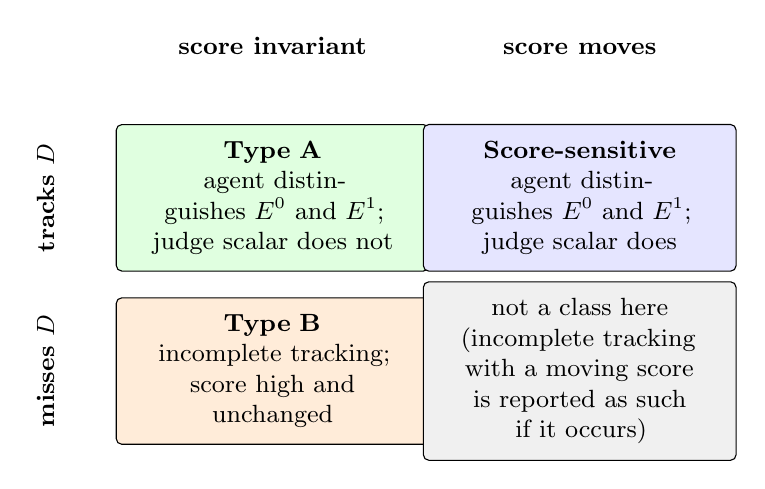
\begin{tikzpicture}[
  box/.style={draw, rounded corners=2pt, align=center, inner sep=6pt,
              text width=3.55cm, font=\small},
  hdr/.style={font=\small\bfseries, anchor=south}
]
\node[hdr] at (2.1,2.55) {score invariant};
\node[hdr] at (6.0,2.55) {score moves};
\node[hdr, rotate=90] at (-0.55,0.85) {tracks $D$};
\node[hdr, rotate=90] at (-0.55,-1.35) {misses $D$};
\node[box, fill=green!12] (A) at (2.1,0.85)
  {\textbf{Type A}\\agent distinguishes $E^0$ and $E^1$;\\judge scalar does not};
\node[box, fill=blue!10] (S) at (6.0,0.85)
  {\textbf{Score-sensitive}\\agent distinguishes $E^0$ and $E^1$;\\judge scalar does};
\node[box, fill=orange!15] (B) at (2.1,-1.35)
  {\textbf{Type B}\\incomplete tracking;\\score high and unchanged};
\node[box, fill=gray!12] (X) at (6.0,-1.35)
  {not a class here\\(incomplete tracking\\with a moving score\\is reported as such\\if it occurs)};
\end{tikzpicture}
\caption{Taxonomy of valid pairs. Rows are agent behavior (final answer
vs.\ gold). Columns are judge behavior (exact $S$). Type~A is not
automatically a rubric bug; Section~\ref{sec:rubric} reads per-criterion
arrays where they exist. Execution failures never occupy this grid.}
\label{fig:taxonomy}
\end{figure}

\paragraph{Classes (valid pairs only).}
\textbf{Type A:} $\mathrm{track}=1$ and $\Delta S=0$.
\textbf{Score-sensitive:} $\mathrm{track}=1$ and $\Delta S\neq 0$.
\textbf{Type B:} $\mathrm{track}=0$ and the score remains high and
unchanged relative to baseline (here: both scores $\ge 80$ and
$\Delta S=0$ on the three primary Type~B cells; ablation/exploratory
Type~B cells are $100{\to}100$).
The unused cell of Figure~\ref{fig:taxonomy} (miss + moving score) is
not observed as a primary headline class in this snapshot.

\paragraph{Universe.}
Ten tasks from one pre-registered eligibility pool (seed
\texttt{20260826}): four Stage-4 locks and six Phase~B additions
(Table~\ref{tab:protocol}). Designed roles were frozen before runs.
Observed class is coded after, against gold, not reverse-fitted to the
design table.

Five lanes: Claude, GPT-5.5, and Qwen3.5-35B-A3B (primary); Qwen3.5-9B
(size ablation); Qwen3.8-Flash (exploratory). Design matrix:
$50$ intended cells. Never scheduled, and \emph{not} execution failures:
Qwen3.5-9B and Qwen3.8-Flash on \task{preference\_inference-f018} and
\task{counterfactual-f004} ($4$ cells, $8$ legs). Executed: $46$ cells,
$92$ legs. Of those legs, $57$ are \texttt{DONE} and $35$ are execution
failures ($15$ of $35$ on Qwen3.5-35B-A3B, mostly \texttt{EMPTY\_XML}).
Valid pairs: $24$. Invariance rate for a model is Type~A / tracking-valid
(Type~B excluded from that denominator). Intervals are exact
Clopper--Pearson $95\%$ CIs. Lanes are never pooled.

\begin{table}[t]
\centering
\small
\caption{Frozen tasks and pre-registered design role. Observed class is
reported in Section~\ref{sec:results}, not in this table.}
\label{tab:protocol}
\begin{tabular}{lll}
\toprule
Task & Phase & Designed role \\
\midrule
\task{retrieval-f001} & A & control \\
\task{aggregation-f003} & A & control \\
\task{preference\_inference-f018} & A & designed Type B (joint $D$) \\
\task{counterfactual-f004} & A & score-sensitive contrast \\
\task{retrieval-f003} & B & control \\
\task{retrieval-f016} & B & control \\
\task{retrieval-f029} & B & control (dual-channel) \\
\task{retrieval-f030} & B & designed Type B \\
\task{aggregation-f018} & B & designed Type B \\
\task{preference\_inference-f004} & B & score-sensitive contrast \\
\bottomrule
\end{tabular}
\end{table}

\section{Results}
\label{sec:results}

The evidence that matters is that all three cells of
Figure~\ref{fig:taxonomy} occur, including on the same task across
agents. Coverage tables follow the examples so that denominators are
defined, not so that a rate can be quoted as the finding.

\subsection{Type A: tracked, score unchanged}
\label{sec:type-a}

All five lanes complete \task{retrieval-f001} (loyalty tier and miles:
Gold/$38{,}450\to$Silver/$8{,}620$) and all five track both legs.
Scores stay at the base value (100 on four lanes; 80 on Qwen3.5-9B).
The rubric does not pin Gold or $38{,}450$. Two correctly reported worlds
can share a score; that is the eligibility design, not a hidden agent
failure.

Claude \task{aggregation-f018} was \emph{designed} as a Type~B trap
(sqlite charitable $\$950\to\$0$ and home-office $104\to 0$ days; W-2/1099
and paired files held). Claude is the only lane that completed both
legs (GPT's CF leg is \texttt{EMPTY\_XML}). Observed class is
\textbf{Type A}: CF zeroes both sqlite fields, holds the untouched file
figures, and flags the file/sqlite mismatch. Score $100\to 100$. This is
the cleanest positive control in the audit: joint $D$ tracked, distractor
channel correctly not moved.

Other primary Type~A pairs (both legs match gold; $\Delta S=0$): Claude
\task{retrieval-f003} $65\to 65$ ($\$136{,}320\to\$80{,}000$);
\task{retrieval-f016} $100\to 100$; \task{retrieval-f029} $100\to 100$;
\task{aggregation-f003} $80\to 80$. GPT \task{retrieval-f001},
\task{retrieval-f003} $100\to 100$, \task{aggregation-f003} $50\to 50$.
Qwen3.5-35B-A3B only on \task{retrieval-f001} $100\to 100$.

\subsection{Score-sensitive: tracked, score moves}
\label{sec:score-sensitive}

\task{preference\_inference-f004} flips HangryDash's top restaurant from
Cooper's Seafood House (88 orders) to Backyard Ale House (59), with
TableFind held. Claude and GPT both report the flip and leave TableFind
unchanged. Scores drop $100\to 79$ (Claude) and $100\to 58$ (GPT) because
the rubric pins Cooper's as HD top. Tracking succeeded; the judge
responded. That is the opposite of Type~B.

GPT additionally tracks three retrieval interventions whose scores move
anyway: \task{retrieval-f016} $100\to 85$ (cost basis
$\$8{,}213.25\to\$7{,}114.20$, cash $\$420\to\$50$);
\task{retrieval-f029} $33\to 100$ (W-2 $\$142\mathrm{k}/\$28.4\mathrm{k}
\to\$90\mathrm{k}/\$18\mathrm{k}$; per-criterion arrays attribute the
swing to items other than the wage figure);
\task{retrieval-f030} $53\to 100$ (TY2025 1099 held at $\$1{,}200$;
charitable $\$950\to\$100$, file/sqlite mismatch flagged). Same agent,
same protocol: Type~A and score-sensitive co-exist.

\subsection{Type B: incomplete tracking, score holds}
\label{sec:type-b}

Re-read against final DONE text and guest gold:

\begin{enumerate}[leftmargin=1.4em,itemsep=0.4em]
\item \textbf{Claude \task{retrieval-f030}, $100\to 100$.}
Designed move is sqlite charitable $\$950\to\$100$ with TY2025 1099 held
at $\$1{,}200$. Base DONE answers \emph{filed TY2024} 1099-NEC
$\$1{,}080$, not the determining TY2025 $\$1{,}200$. CF reports
$\$1{,}200$ and charitable $\$100$. Type~B is the base-leg wrong year,
not a CF miss of charitable.
\item \textbf{Claude \task{preference\_inference-f018}, $100\to 100$.}
Joint $D$: GME $85\to 0$ and OddsMarket YES $200$/active $\to 0$/settled.
CF lists GME $0$ shares / $\$0$ basis, and still lists GameStop YES as
$200$ shares / $\$16.00$ (same as base). One conjunct tracked; the joint
set is not. Cleanest Type~B.
\item \textbf{GPT \task{counterfactual-f004}, $87\to 87$.}
Guest zeroes the 1099 amount. CF still reports a $\$1{,}200$ stipend and
$\$1{,}068$/year net. Not an execution failure; Claude's base leg on
this task is not \texttt{DONE}.
\end{enumerate}

Ablation/exploratory Type~B (not primary): Qwen3.5-9B
\task{retrieval-f016} base reports $\$8{,}788.75$ vs.\ gold
$\$8{,}213.25$ (CF exact $\$7{,}114.20$), scores $100\to 100$;
Qwen3.8-Flash \task{retrieval-f029} CF ``Total Income $\$91{,}200$'' vs.\
Box~1 gold $\$90{,}000$ (withholding $\$18{,}000$ exact), scores
$100\to 100$.

\subsection{Designed role vs.\ observed class}

Pre-registration does not fix the outcome. \task{aggregation-f018}
(designed Type~B) $\to$ Claude Type~A. \task{retrieval-f030} (designed
Type~B) $\to$ Claude Type~B and GPT score-sensitive. 
\task{preference\_inference-f018} (designed Type~B) $\to$ Claude Type~B
as specified. \task{preference\_inference-f004} (designed sensitive)
$\to$ Claude and GPT sensitive. \task{counterfactual-f004} (designed
sensitive) $\to$ GPT Type~B: the intervention moved; the answer did not.

\subsection{Per-model counts}
\label{sec:counts}

\begin{table}[t]
\centering
\small
\caption{Primary tier. Invariance $=$ Type~A / tracking-valid. CI is
exact Clopper--Pearson $95\%$. $n\le 9$; intervals are wide by
construction.}
\label{tab:primary}
\begin{tabular}{lrrrrrrl}
\toprule
Model & Valid & Tracking-valid & Type A & Sensitive & Type B & Invariance & 95\% CI \\
\midrule
Claude & 9 & 7 & 6 & 1 & 2 & 0.857 & [0.421, 0.996] \\
GPT & 8 & 7 & 3 & 4 & 1 & 0.429 & [0.099, 0.816] \\
Qwen3.5-35B-A3B & 1 & 1 & 1 & 0 & 0 & 1.000 & [0.025, 1.000] \\
\bottomrule
\end{tabular}

\end{table}

\begin{table}[t]
\centering
\small
\caption{Ablation and exploratory tiers. Not pooled with Table~\ref{tab:primary}.}
\label{tab:ablation}
\begin{tabular}{lrrrrrrl}
\toprule
Model & Valid & Track. & A & Sens. & B & Inv. & 95\% CI \\
\midrule
Qwen3.5-9B & 3 & 2 & 1 & 1 & 1 & 0.500 & [0.013, 0.987] \\
Qwen3.8-Flash & 3 & 2 & 1 & 1 & 1 & 0.500 & [0.013, 0.987] \\
\bottomrule
\end{tabular}
\end{table}

\begin{figure}[t]
\centering

\includegraphics[width=0.58\linewidth]{score_pairs_primary.png}
\caption{Primary valid pairs: $S^0$ vs.\ $S^1$. Diagonal: invariant.
Off-diagonal: score-sensitive. Type~B points track incompletely despite
the score.}
\label{fig:score-pairs-primary}
\end{figure}

\begin{figure}[t]
\centering

\includegraphics[width=0.55\linewidth]{invariance_by_tier.png}
\caption{Per-model invariance among tracking-valid pairs. Bars are not a
pooled rate.}
\label{fig:invariance}
\end{figure}

Table~\ref{tab:primary} is the reportable unit. Qwen3.5-35B-A3B's $1/1$
is execution coverage (nine of ten cells fail), not an invariance
finding.

\subsection{Judge vs.\ agent: rubric arrays}
\label{sec:rubric}

On \task{aggregation-f003} ($\$4{,}871.70\to\$400$), four completing
lanes track both totals. Claude and GPT are Type~A; 9B and Flash are
score-sensitive. GPT stays at \texttt{[1,1,0,0]} both legs: the
refund-linked criteria pass twice; year-count/format criteria never
fire. 9B moves \texttt{[1,1,0,0]}$\to$\texttt{[1,1,1,0]}; Flash
\texttt{[1,1,1,0]}$\to$\texttt{[1,1,1,1]} --- one extra criterion under
CF, not a change in the reported total. Type~A here is not ``the refund
criteria were blind.'' Score-sensitive here is not ``the agent failed to
track.''

\subsection{Cells outside this universe}

\task{hard\_app-f033} and \task{situated\_action-f028} are pilot-only
and unaudited. No trajectory, guest file, patch, or writer output was
modified to produce these numbers.

\section{Discussion}

Completion scores measure termination plus whatever the rubric binds.
They do not, by themselves, measure whether $D$ was read, and they do
not, by themselves, measure whether $J$ is attached to $D$. Type~A shows
the first without the second; score-sensitive shows both; Type~B shows
completion (and a high score) without tracking. That is the distinction
this protocol is for.

Score invariance is not a defect to be patched out of every rubric. A
channel-invariant item that asks whether the agent used the right app
and reported \emph{a} value can award the same score to two correct
worlds (\task{retrieval-f001}). Changing that rubric would change the
task. The audit's job is to make the binding visible.

Designed traps are hypotheses, not labels. Reporting only the
pre-registered role would have mis-stated Claude \task{aggregation-f018}
and would have collapsed Claude and GPT on \task{retrieval-f030}.

\section{Related work}

OSWorld~\citep{xie2024osworld}, WebArena~\citep{zhou2024webarena}, and
VisualWebArena~\citep{koh2024visualwebarena} score agents with
completion rubrics. MyPCBench~\citep{jang2026mypcbench} seeds a personal
desktop that our $I$ reuse. None of these leaderboards pair $E^0$ with
$E^1=I(E^0)$ to split tracking from $S$.

\citet{shao2026protocolvalidity} argue that a benchmark score supports a
capability claim only when the intended capability remains necessary for
success, and they audit shortcut paths. We audit a different cut: whether
a gold-moving intervention that the guest confirms is reflected in the
answer and in $S$. Complementary, not equivalent.
\citet{turk2026counterfactualclinical} pair clinical cases with
controlled mutations and find that coverage-style scores can hide
update failures; we observe the same \emph{pattern} (score vs.\ state
change) for GUI CUAs on personal-data tasks.
\citet{bellibatlu2026judgesense} measure judge instability under prompt
paraphrase; we measure judge (in)sensitivity to a verified world-state
change, using the rubric's own item array when available.

The pairing $E^1=I(E^0)$ follows the interventionist language of
\citet{pearl2009causality}. We do not identify internal causal
structure of the model.

\section{Limitations}

Ten tasks, one environment, five lanes, $n\le 9$ valid pairs per primary
model. CIs are wide; they bound binomial uncertainty on this sample,
not a deployment rate. Qwen3.5-35B-A3B contributes one semantic pair.
Classification of all $24$ valid pairs is hand-coded from final-answer
text against guest gold (\texttt{tracking\_evidence.md}); traceable, not
automated. Score deltas are attributed to rubric items only where
\texttt{per\_rubric\_max} exists. Interventions test evaluator and agent
behavior under controlled state changes, not arbitrary real-world
shifts.

\section{Conclusion}

On this frozen audit, task completion, counterfactual tracking, and
benchmark score sensitivity come apart. A stable score does not certify
tracking; a moving score does not certify a tracking failure. Paired,
gold-moving checks make that split observable. CUA leaderboards
currently do not run them.

\bibliographystyle{plainnat}
\bibliography{references}

\end{document}
